\section{Description of different components}
\label{Description-components}
This section gives a general description of different components involved in DINO code. The two most important components in DINO are source files which contain different modules and input files for specific applications. In the following text, these two parts are introduced in detail.
\subsection{Modules contained in {\it DINO}}
All the modules contained in DINO are located in \textit{\$DINOSOARS\_HOME/SOURCES/} directory, the detailed description of these modules are as follows:
\begin{itemize}
  \item \textbf{MAIN}: It contains only one subroutine \textbf{dinosoars.f90}, which is the main function. Everything starts here and ends here.
  \item \textbf{INIT}: It contains all the subroutines for initialization. Different initial profiles are included in the subdirectory \textit{INIT\_PROFILES/}.
  \item \textbf{MODULES}: It contains module files defining most of the variables used in DINO and namelist sections of the input file (DINO\_IN).
  \item \textbf{MESH}: It contains mesh generation module, including all the variables and functions releted to mesh generation.
  \item \textbf{FLOW\_FIELD}: It contains all subroutines computing variables related to flow field.
  \item \textbf{THERMODYNAMICS}: It contains all subroutines computing thermodynamical properties.
  \item \textbf{TRANSPORT}: It contains all subroutines related to transport properties computation.
  \item \textbf{CHEMISTRY}: It contains all subroutines related to chemical reaction computation.
  \item \textbf{FPI}: It contains subroutines which compute thermodynamics properties, transport properties and reaction rate based on tabulated flame table instead of cantera or Eglib \cite{ern_1994,ern_1995}.
  \item \textbf{TURBULENCE}: It contains all the subroutines involved in the implementation of the pseudo turbulence fields.
  \item \textbf{ODT}:
  \item \textbf{PREPARE\_RHS}: It contains subroutines which computes the right-hand-side used during the integration procedure.
  \item \textbf{RHS}: It contains subroutines computing the right-hand-side of each individual governing equation. These subroutines are coupled in the general subroutines in PREPARE\_RHS.
  \item \textbf{DERIV}: It contains all the subroutines you need to compute x, y and z first and second derivatives.
  \item \textbf{RUNGE\_KUTTA}: It contains subroutines where different time itegration schemes are implemented.
  \item \textbf{POISSON}: It contains subroutines you need to compute pressure and poisson equation.
  \item \textbf{2DECOMP}: It contains all the subroutines related to the use of FFT library.
  \item \textbf{PARALLEL}: It contains all the subroutines needed to work in parallel.
  \item \textbf{BOUNDARY}: It contains all that you need to implement various kinds of boundary conditions.
  \item \textbf{IBM}: It contains all subroutines for the immersed boundary implementation.
  \item \textbf{TWOPHASE}: It contains all the subroutines for the computation of two phase flow.
  \item \textbf{UTILS}:
  \item \textbf{CEQ}:
  \item \textbf{DCS}:
  \item \textbf{INCLUDE}:
  \item \textbf{EGLIB}: It contains all that you need to compute the volume viscosity transport term using the eglib library.
  \item \textbf{CHEMKIN}: It contains subroutines associated with the CHEMKIN chemical library.
  \item \textbf{ERRORS}: It contains the error analysis module.
  \item \textbf{SAVE}: It contains all that you need to save and read results.
  \item \textbf{flameletconfig}:
\end{itemize}
A flow chart of DINO is given in Fig.~\ref{fig:flowchart}
\begin{figure*}[htbp]
\centering
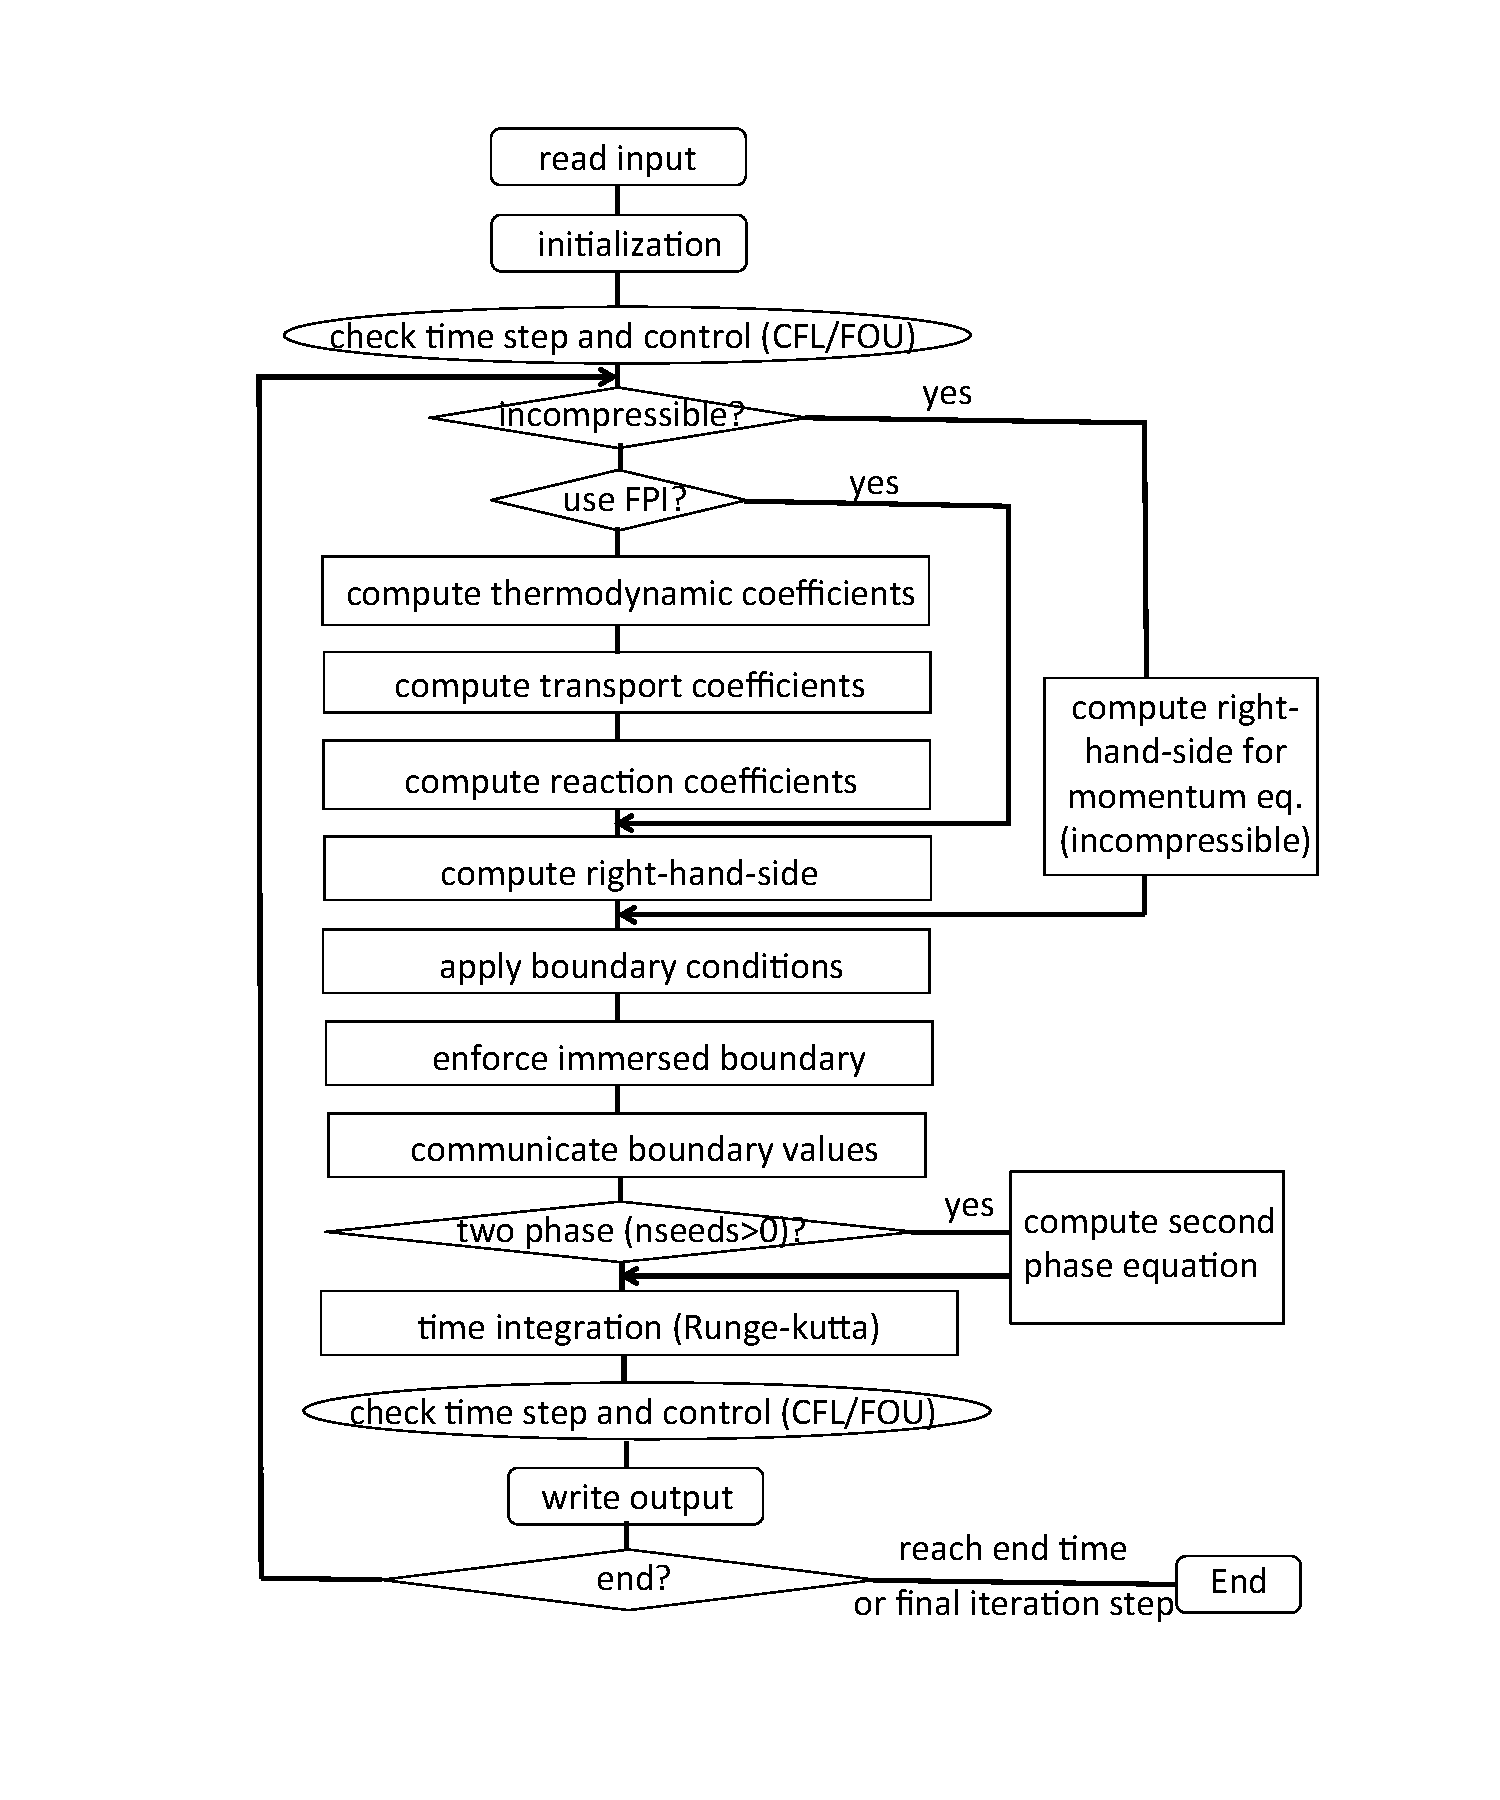
\includegraphics[width=\textwidth]{chart}
\caption{Flow chart of DINO}
 \label{fig:flowchart}
\end{figure*}

\subsection{Description of the input file}
The input file for DINO is named as \textit{DINO\_IN}, this file contains all the information needed by DINO to do a run. It corresponds to the module files (*\_mod.f90) present in \textit{\$DINOSOARS\_HOME/SOURCES/MODULES}. The example input files can be found in the WORK directory \textit{\$DINOSOARS\_HOME/WORK/RUNS/}. Now we will describe the input file in details:
\begin{itemize}
  \item NML\_INITIALIZE (module subroutine dino\_init\_mod.f90): contains the initial conditions for the simulation.
  \begin{lstlisting}
    &NML_INITIALIZE
        INIT_TYPE=1,
        USE_COMPACT=.FALSE.,
        INIT_PRESSURE=101325.D0,
        INIT_TEMPERATURE=300.D0,
        JET_FLOW_DIR = 1,
        INIT_XVEL=0.016D0,
        INIT_YVEL=0.D0,
        INIT_ZVEL=0.D0,
        INIT_VEL_JET=0.D0,
        INIT_VEL_COFLOW=0.D0,
        INIT_VEL_START=0,
        RADIUS=5.D-2,
        STIFF=0.5D3,
        STRAIN_RATE=0.D0,
        INIT_TEMP_JUMP=1.D3,
        INIT_VEL_JUMP=0.D0,
        CONST_RHO=1.177D0,
        CONST_MU=1.846D-5,
        GAS_PHASE(1)='air_cold',
        GAS_PHASE(2)='O2:1.0, N2:3.7619',
        GAS_PHASE(3)='',
        EQUI_RATIO=0.0,
        SPECIES_FUEL(1)='O2',
        SPECIES_FUEL(2)='O2',
        SPECIES_PROD(1)='O2',
        SPECIES_PROD(2)='O2',
        SPECIES_INERT(1)='N2'
  \end{lstlisting}
  INIT\_TYPE defines the category of the initial profile for your specific application. See \textit{SOURCES/INIT/dino\_init\_sol.f90} for a detailed and up-to-date list of all you can choose. USE\_COMPACT chooses 6th order compact difference scheme instead of the 6th order explicit finite difference scheme if turned on, it is still IN TEST. INIT\_PRESSURE is the initial pressure, INIT\_TEMPERATURE is the initial temperature, INIT\_XVEL, INIT\_YVEL and INIT\_ZVEL are the initial x, y, and z-velocities. JET\_FLOW\_DIR is the direction of the jet flow (1-x, 2-y, 3-z). INIT\_VEL\_JET is the initial velocity of the jet flow, INIT\_VEL\_COFLOW is the initial velocity of the coflow, RADIUS defines the radius of the jet flow cross-section, STIFF defines the stiffness between the jet flow and coflow. INIT\_VEL\_START defines the variable to start coupling between initial velocity and temperature. If INIT\_VEL\_START is larger than 1, it means the chemistry will start without velocity. INIT\_TEMP\_JUMP is the temperature difference between fresh and burnt gas mixture, if it is defined as 0, the temperature difference will be computed from equilibrium. INIT\_VEL\_JUMP is the velocity difference. CONST\_RHO defines the constant density for incompressible flow, CONST\_MU defines the constant viscosity. GAS\_PHASE(1) is the name of the chosen gas chemistry mechanism, the user will find all other existing chemistry mechanism in directory \textit{\$DINOSOARS\_HOME/WORK/MECHANISMS}. The user can also introduce any other chemistry mechanism with format *.cti or *.xml in the MECHANISMS directory and use it for the simulation. GAS\_PHASE(2) defines the composition of the gas for the simulation. GAS\_PHASE(3) ???. EQUI\_RATIO when is it used???. SPECIES\_FUEL(1) defines the first fuel, SPECIES\_FUEL(2) defines the second fuel, SPECIES\_PROD(1) defines the first product, SPECIES\_PROD(2) defines the second product, SPECIES\_INERT(1) defines the inert gas.
  \item NML\_SCALARS (module subroutine dino\_scalars\_mod.f90): contains user-defined scalar variables, it is used for further development of the code.
  \begin{lstlisting}
    &NML_SCALARS
        NSCAL=0,
        NAMES(1)='MixFrac',
        IS_REACTIVE(1)=.false.
  \end{lstlisting}
  NSCAL is the number of user-defined scalar variables.
  \item NML\_TIME\_INTEGRATION (module subroutine dino\_time\_integration\_mod.f90): contains the time integration method and related control parameters.
  \begin{lstlisting}
    &NML_TIME_INTEGRATION
        INTEGRATION_SCHEME=1,
        RK_TIME_STEP_CONTROL=.false.,
        RK_DT_CONTROL_ACCURACY=0.8D-3,
        RK_DT_CONTROL_INTERVAL=200,
  \end{lstlisting}
  INTEGRATION\_SCHEME determines which time integration method to use, 1 represents fully explicit 4th order Runge-Kutta method, 2 represents semi-implicit 3rd order Runge-Kutta, Rosenbrock method, 3 represents additive semi-implicit 4th order Runge-Kutta with RADAU-5 method. RK\_TIME\_STEP\_CONTROL chooses whether to turn on Runge-Kutta time step control. If RK\_TIME\_STEP\_CONTROL is true, the doubling error between integration scheme 1 and 2 will be computed every RK\_DT\_CONTROL\_INTERVAL steps, then compared with the defined accuracy RK\_DT\_CONTROL\_ACCURACY to control the time step in the fully explicit 4th order Runge-Kutta method.
  \item NML\_CONTROL (module subroutine dino\_control\_mod.f90): contains parameters for time step control.
  \begin{lstlisting}
    &NML_CONTROL
        INIT_TIMESTEP=1.D-5,
        TIME_STEP_CTRL_START=10,
        TSTEP_MIN=1.0D-10,
        TSTEP_MAX=1.D-2,
        TIME_END=1.25D,
        ITE_END=10000,
        RANDOMSEEDS=.true.,
        CFL_LIM=0.25D0,
        CFL_CTRL=.true.,
        FOU_LIM=0.5D0,
        FOU_CTRL=.true.,
        DEBUG_LOCAL=.false.,
        DEBUG_END_ITE=20
  \end{lstlisting}
  INIT\_TIMESTEP is the initial time step at the begining of the simulation. TIME\_STEP\_CTRL\_START defines from which step the time step control begin. TSTEP\_MIN is the minimal time step allowed, TSTEP\_MAX is the maximum time step allowed. TIME\_END is the end time for the simulation, ITE\_END is the end iteration step for the simulation. RANDOMSEEDS make sure the fluctuation is random if true. CFL\_LIM is the CFL time step control delimeter, CFL\_CTRL determines whether to use CFL time step control. FOU\_LIM is the Fourier time step control delimeter, FOU\_CTRL determines whether to use Fourier time step control. DEBUG\_GLOBAL print out 3D array entries if true. DEBUG\_LOCAL print out to stdout debuging information for DEBUG\_END\_ITE iterations.
  \item NML\_DIMENSIONS (module subroutine dino\_dimensions\_mod.f90): contains the domain and grid information.
  \begin{lstlisting}
    &NML_DIMENSIONS
        LENGTH_X=0.5D0,
        LENGTH_Y=0.5D0,
        LENGTH_Z=1.D0,
        DIMX_TOTAL=71,
        DIMY_TOTAL=71,
        DIMZ_TOTAL=1
  \end{lstlisting}
  LENGTH\_X, LENGTH\_Y, LENGTH\_Z are the domain size in x, y, z direction respectively. DIMX\_TOTAL, DIMY\_TOTAL, DIMZ\_TOTAL are the grid number in x, y, z direction repectively. DIMZ\_TOTAL=1 means 2D or 1D case, DIMY\_TOTAL=1 means 1D case. For higher FFT efficiency and less numerical polution, DIMX\_TOTAL should be odd number if it is non-periodic boundary condition in x direction, even number if periodic boundary condition. It is the same case for DIMY\_TOTAL and DIMZ\_TOTAL.
  \item NML\_BOUNDARY (module subroutine dino\_boundary\_mod.f90): contains the boundary conditions.
  \begin{lstlisting}
    &NML_BOUNDARY
        BC_LEFT=1,
        BC_RIGHT=8,
        BC_UP=4,
        BC_DOWN=4,
        BC_FRONT=3,
        BC_BACK=3,
        BC_VEL_INLET=.false.,
        U_IN_CTRL=.FALSE.,
        P_INFTY=101325.0D0
  \end{lstlisting}
  BC\_LEFT, BC\_RIGHT, BC\_UP, BC\_DOWN, BC\_FRONT, BC\_BACK defines the boundary condition for left, right, up, down, front, back side of the computational domain respectively.
  Different boundary conditions are represented by different numbers:
  \begin{lstlisting}
    #artificial        = 0
    #subsonic_inlet    = 1
    #subsonic_outlet   = 2 > the outlet pressure equals to atmosphere pressure
    #periodic          = 3
    #symmetry          = 4
    #adiabatic_wall    = 5
    #isothermal_wall   = 6
    #moving_wall       = 7
    #outlet_flow       = 8 > the normal derivative of pressure equals to 0
    #mixed_bc          = 9 > mixed boundary condition
  \end{lstlisting}
  BC\_VEL\_INLET is true if the inlet velocity is not constant and defined by the user. U\_IN\_CTRL is used for x-velocity control during flame speed computation. P\_INFTY defines the atmosphere pressure.
  \item NML\_IMMERSED\_BOUNDARY (module subroutine dino\_ib\_mod.f90): contains the immersed boundary information
  \begin{lstlisting}
    &NML_IMMERSED_BOUNDARY
        IB_GEOMETRY=.FALSE.,
        IB_GHOST=.TRUE.,
        USE_3RD_IB=.FALSE.
        IB_XVEL=0.D0,
        IB_YVEL=0.D0,
        IB_ZVEL=0.D0,
        IB_WVEL=0.D0,
        IB_DATA='circular_cylinder.dat',
        IB_DATA_TYPE=0,
        PROJECTION_POINTS=1,
        IB_FLOW='external_flow'
  \end{lstlisting}
  There are two different immersed boundary methods the user can choose for complex geometry. One is direct boundary IBM, the other is ghost-cell IBM.
  IB\_GEOMETRY determines whether to activate the direct boundary immersed boundary method. IB\_DATA is the binary data file for a specific geometry, IB\_DATA\_TYPE is the geometry data type, 0 for eulerian data, 1 for lagrangian data. PROJECTION\_POINTS determines the interpolation order. IB\_FLOW determines whether the flow is internal or external;
  IB\_GHOST determines whether to activate ghost-cell immersed boundary method. (Ghost-cell IBM is still in development). USE\_3RD\_IB determines whether to use 3rd order ghost-cell IBM, 2nd order if false. IB\_XVEL, IB\_YVEL, IB\_ZVEL and IB\_WVEL is the x, y, z-velocity and rotating velocity of the moving geometry respectively.
  More details introducing IBM are in the next chapter.
  \item NML\_POISSON\_SOLVER (module subroutine dino\_poisson\_solver\_mod.f90): contains information about poisson solver.
  \begin{lstlisting}
    &NML_POISSON_SOLVER
        PRESSURE_SPECTRAL_SOLVER=.TRUE.,
        INCOMPRESSIBLE=.TRUE.,
        PGRADX=.FALSE.,
        PGRADY=.FALSE.,
        PGRADZ=.FALSE.,
        PRESSURE_FFT_LIB=1,
        SUPPRESS_NOISE_X=.FALSE.,
        SUPPRESS_NOISE_Y=.FALSE.,
        SUPPRESS_NOISE_Z=.FALSE.,
        REMOVE_MEAN_PRESSURE=.FALSE.
  \end{lstlisting}
  PRESSURE\_SPECTRAL\_SOLVER solve pressure term with fully spectral method if true. INCOMPRESSIBLE is true when using fully incompressible solver. PGRADX, PGRADY and PGRADZ are constant pressure gradient in x, y and z direction respectively. Constant pressure gradient works only with poiseuille flow. PRESSURE\_FFT\_LIB chooses the FFT library, 1 represents 2decomp library, 2 represents standard fftw3 library without 2decomp.

  \item NML\_RESTART (module subroutine dino\_restart\_mod.f90): contains the restart file information to restart the simulation half-way.
  \begin{lstlisting}
    &NML_RESTART
        RESTART=.FALSE.,
        RESTART_TAG='1500',
        DINO_NEW_TIME_STEP=.TRUE.,
        READ_FROM_1D=.FALSE.,
        TWOD_FROM1D=.FALSE.,
        THREED_FROM1D=.FALSE.,
        THREED_FROM2D=.FALSE.,
        PATCH_SOLUTION=.FALSE.,
        PATCH_ITERATION=3000,
        PATCH_SOL_FILE=''
  \end{lstlisting}
  RESTART determines whether the simulation starts from the begining or starts from a specific iteration step defined in RESTART\_TAG. DINO\_NEW\_TIME\_STEP determines whether to use the new initial time step or keep the original one when restart the simulation. READ\_FROM\_1D should be turned on if you want to project a 1D simulation into 3D. PATCH\_SOLUTION, PATCH\_ITERATION, PATCH\_SOL\_FILE ???
  \item NML\_REACTION (module subroutine dino\_reaction\_mod.f90): contains information about reaction.
  \begin{lstlisting}
    &NML_REACTION
        REACTIVE=.FALSE.,
        REACTION_START_IT=1,
        PHYSCHEM_LIB=1,
        IGN_INTENSITY=0.0D2,
        IGN_DURATION=0.D-6,
        IGN_LENGTH=0.D-4,
        TEMPER_TH=0.D0,
        USE_FPI=.FALSE.,
        READ_BINARY=.false.,
        FORCING=.TRUE.,
        Y_FORCING_TYPE=0
  \end{lstlisting}
  REACTIVE is true when consider reaction in the flow simulation. REACTION\_START\_IT determines from which iteration step reaction is considered. PHYSCHEM\_LIB is 1 when use cantera for chemical reaction computation. At present, other options for PHYSCHEM\_LIB are not stable. USE\_FPI is true when use FPI chemistry table instead of detailed chemistry mechanism for the computation. READ\_BINARY is false if the FPI table is txt data, true if binary data. TEMPER\_TH ??? FORCING is true if you want to ensure the summation of all species mass fraction is equal to 1. Y\_FORCING\_TYPE determines which forcing method to use. 0 means normalizing all the species mass fractions; 1 means computing all species mass fractions except one inert gas species (usually N2), the mass fraction of that inert gas species is computed by 1 - sum(mass fraction of all other species).
  \item NML\_TRANSPORT (module subroutine dino\_transport\_mod.f90): contains transport information.
  \begin{lstlisting}
    &NML_TRANSPORT
        MOLTRANS_LIB=1,
        DIF_SORET=.FALSE.,
        DIF_DUFOUR=.FALSE.,
        DIF_MULTI=.FALSE.,
        DIF_ULEWIS=.FALSE.,
        VOL_VISC=.FALSE.,
        EGLIB_MODEL_NUM=2,
        EGLIB_SCALE_FACTOR=1.D0,
        VISCOSITY_CTRL=.FALSE.
  \end{lstlisting}
  MOLTRANS\_LIB is 1 when use cantera for transport computation, 5 when use EGlib for transport computation. Other options are not recommended. DIF\_SORET activates thermal diffusion (Soret effect) in the computation. When light species such as H2 is considered as a fuel, soret effect should be turned on. DIF\_DUFOUR activates dufour effect in the computation. DIF\_MULTI activates multi-component diffusion while the default is mixture-averaged diffusion. DIF\_ULEWIS takes unity Lewis number assumption for diffusion velocity. VOL\_VISC is the volume viscosity activation boolean.
  \item NML\_GRAVITY (module subroutine dino\_gravity\_mod.f90)
  \begin{lstlisting}
    &NML_GRAVITY
        GRAVITY_X=0.D0,
        GRAVITY_Y=0.D0,
        GRAVITY_Z=0.D0
  \end{lstlisting}
  GRAVITY\_X, GRAVITY\_Y and GRAVITY\_Z define the gravity force in x, y and z direction respectively.
  \item NML\_GRIDDING (module subroutine dino\_grid\_mod.f90): contains parameters on mesh grid.
  \begin{lstlisting}
    &NML_GRIDDING
        XGRID_TYPE=1,
        YGRID_TYPE=1,
        ZGRID_TYPE=1,
        TAU_STR_CENTER_X=2.D0,
        TAU_STR_CENTER_Y=2.D0,
        TAU_STR_CENTER_Z=2.D0,
        REF_CENTER_X=5.D-3,
        REF_CENTER_Y=6.D-3,
        REF_CENTER_Z=2.D0,
        BETA_G_BOUND=0.5D0
  \end{lstlisting}
  XGRID\_TYPE, YGRID\_TYPE and ZGRID\_TYPE are defining the grid type in x, y, z directions. There are 3 types of grid: 1 represents regular grid, 2 represents center refined grid, 3 represents boundary refined grid. TAU\_STR\_CENTER\_X, TAU\_STR\_CENTER\_Y and TAU\_STR\_CENTER\_Z are stretching values for center refined grid in x, y, z directions. REF\_CENTER\_X, REF\_CENTER\_Y and REF\_CENTER\_Z are locating the center of refinement. BETA\_G\_BOUND is the stretching value for boundaries refined grid.
  \item NML\_PARAMETERS (module subroutine dino\_parameters\_mod.f90)
  \begin{lstlisting}
    &NML_PARAMETERS
        CLOSED_DOMAIN=.FALSE.
  \end{lstlisting}
  CLOSED\_DOMAIN is true if the domain is bounded by wall boundary condition at all sides.
  \item NML\_VORTEX (module subroutine dino\_add\_vortex\_mod.f90)
  \begin{lstlisting}
    &NML_VORTEX
        VORT_NUMB=0,
        VORT_CENTX(1)=0.5D-2,
        VORT_CENTX(2)=0.0D0,
        VORT_CENTY(1)=0.5D-2,
        VORT_CENTY(2)=0.0D0,
        VORT_CENTZ(1)=0.D0,
        VORT_CENTZ(2)=0.D0,
        VORT_RAD(1)=0.2D-3,
        VORT_RAD(2)=0.D0,
        VORT_STRENGTH(1)=0.D0,
        VORT_STRENGTH(2)=0.D0
  \end{lstlisting}
  The parameters and options in this section are for votex study.
  \item NML\_TWOPHASE (module subroutine dino\_two\_phase\_mod.f90): description of variables for two phase flow.
  \begin{lstlisting}
    &NML_TWOPHASE
        NSEEDS=0,
        TYPE_SEEDS=3,
        TWOPHASE_INIT_TYPE=10,
        DENS_SEEDS=684.0D0,
        DIAM_SEEDS=0.025D0,
        TCRITICAL=540.13,
        TBOILING=371.53,
        LATENT_HEAT_MOL=31.8D3,
        WD_OX=0.032D0,
        WD_FUEL=0.1D0,
        CPLIQUID=2260.4D0,
        DETAIL_DROPLET_TRANSPORT_PRO=.TRUE.,
        DINO_DROPLET_MINIMUM_DIAM=1.D-6,
        INIT_TEMPERATURE_SEEDS=300,
        INIT_SEEDS_VELX=0.D0,
        INIT_SEEDS_VELY=-0.01D0,
        INIT_SEEDS_VELZ=0.D0,
        COLLISION_STIFF=5.D3,
        TWO_WAY_COUPLING=.TRUE.,
        TWO_WAY_START_IT=1,
        MASS_TRANSFER=.TRUE.,
        SURFACEPOINT_MANUALLY=.TRUE.,
        NSURFPOINT=400,
        FORCING_TYPE=1
  \end{lstlisting}
  NSEEDS is the number of seeds. If it is 0, no discrete phase will be considered. TYPE\_SEEDS determines the type of the seeds. 0 corresponds to tracer; 1 represents point force solid particles; 2 represents non-resolved droplets; 3 represents resolved sphere; 4 represents resolved fixed object.
  TWOPHASE\_INIT\_TYPE describes the configuration of the twophase flow. The following are different types:
  \begin{lstlisting}
    0 ----> random distribusion of particles;
    1 ----> particles move up;
    2 ----> particles move down;
    3 ----> cluster sheet in the center;
    4 ----> cluster sheet move as jet;
    5 ----> temporally evolving jet of particles, randomly distributed;
    6 ----> spherical cloud of droplets;
    7 ----> jet inlet spray (not available at present);
    8 ----> two particles collide;
    9 ----> one particle in the center;
    10 ---> fixed object
  \end{lstlisting}
  DENS\_SEEDS defines the density of the seeds. DIAM\_SEEDS is the diameter of the seed. TCRITICAL defines the critical temperature, while TBOILING defines the boiling temperature. LATENT\_HEAT\_MOL is the molar latent heat of evaporation. WD\_OX and WD\_FUEL define the molecular weight of the oxidizer and fuel respectively. CPLIQUID is the liquid droplet specific heat at the droplet temperature. DETAIL\_DROPLET\_TRANSPORT\_PRO is false when work with constant liquid/gas properties in order to reduce the numerical cost due to interpolation. DINO\_DROPLET\_MINIMUM\_DIAM defines the minimum possible diameter for droplet, if the size is smaller than this limit, it will be treated as tracer. INIT\_TEMPERATURE\_SEEDS defines the initial temperature for the seeds. INIT\_SEEDS\_VELX, INIT\_SEEDS\_VELY and INIT\_SEEDS\_VELZ define the initial x, y, z velocity of the seeds. COLLISION\_STIFF is the collision stiffness. TWO\_WAY\_COUPLING is true if the turbulence and particles have effect on each other. If TWO\_WAY\_COUPLING is false, it means one way coupling is used, the turbulence can influence the particles, while the particles cannot influence the turbulence.
  TWO\_WAY\_START\_IT is the iteration step from which two way coupling starts. MASS\_TRANSFER is the option to allow mass transfer in the flow or not. SURFACEPOINT\_MANUALLY decide whether manually input or calculate the surface points. NSURFPOINT is the number of the point on the surface + 1 (center of the object). FORCING\_TYPE is 1 for fixed bodies and 2 for moving bodies.
  \item NML\_ODT (module subroutine dino\_odt\_mod.f90)
  \begin{lstlisting}
    &NML_ODT
        ODT_ACTIVE=.FALSE.,
        BRNLLI_TRIAL=.FALSE.,
        BRNLLI_TR_STR=1.D-2,
        DINO_RANDOM_ODT=.FALSE.,
        ODT_RAND_CVX=1.5D0,
        ODT_RAND_CTX=5.D-4,
        ODT_RAND_CYX=0.D0,
        DINO_ODT_TCOE=1.D-1,
        DINO_ODT_DEBUG=0,
        DINO_C_EDDY=5.68D0,
        DINO_Z_EDDY=0.14D0
  \end{lstlisting}
  \item NML\_TURBULENCE (module subroutine dino\_turbulence\_mod.f90): contains turbulence parameters.
  \begin{lstlisting}
    &NML_TRUBULENCE
        INIT_TURBU=.FALSE.,
        TURBU_METHOD=1,
        TURBU_FORCING=.FALSE.,
        SPECTRUM_ANALY_TYPE=1,
        UPRIME=0.D0,
        EPS_KARMAN=0.7D-5,
        IFFT_LE=0.25D-2,
        IFFT_LD=0.2D-3,
        L_INTEG=0.5D-3,
        L_RELAX=0.5D0,
        FTI=.FALSE.,
        FTI_PLANE=1,
        FTI_DOMAIN=1,
        FTI_GENERATION=.FALSE.,
        FTI_DIRECT=.FALSE.
        FTI_FILE='0',
        FILT_FLUCT=.FALSE.,
        FILT_WIDTH=4.D-3,
        DELTA_T=1.D-9,
        COMPUTE_ITE=.FALSE.,
        FOU_LIM_FLUCT=0.02,
        N_ITERATION=10,
        NMODE=1000,
        LE=8.D-5
  \end{lstlisting}
  INIT\_TURBU determines whether to enforce turbulence at the initial step. TURBU\_METHOD is the type of method for generating turbulence. There are 4 turbulence generating methods implemented: 1 represents Inverse Fast Fourier Transform (IFFT) replying on Von Karman spectrum with Pao correction \cite{Parcomb} (VKP spectrum); 2 represents digital filtering method \cite{klein2003}; 3 represents random noise diffusion \cite{kempf2005}; 4 represents Kraichnan technique \cite{Kraichnan1970}.
  \item NML\_SAVING (module subroutine dino\_saving\_mod.f90): contains all parameters for simulation results saving.
  \begin{lstlisting}
    &NML_SAVING
        SAVING_TYPE=1,
        SAVING_RESTART_INTERVAL=250,
        SAVING_AVERAGE_INTERVAL=10000,
        SAVING_CTRL_HDF5_INTERVAL=1,
        SAVING_CTRL_MAX_MIN_INTERVAL=10,
        SAVING_TECPLOT=.false.,
        SAVING_HDF5=.true.,
        SAVING_MPIIO=.true.,
        SAVING_VORTICITY=.FALSE.,
        SAVING_QCRITERION=.TRUE.,
        SAVING_EDDY=.FALSE.,
        SAVING_VISCOSITY=.FALSE.,
        SAVING_VTK=.FALSE.,
        SAVING_TWOPHASE_VTK=.TRUE.,
        SAVING_AVERAGE=.FALSE.,
        SAVING_PLANES=.FALSE.,
        SAVING_PROBES=.FALSE.,
        NPROBES_X=3,
        NPROBES_Y=3,
        NPROBES_Z=1,
        SAVING_TIMES(1)=1.0D-6,
        SAVING_TIMES(2)=1.0D-5,
        SAVE_HEAT_RELEASE=.FALSE.,
        SAVE_MASSFLOW=.FALSE.,
        SAVE_TURBU_PROPS=.FALSE.,
        SAVE_ENERGY_SPEC=.FALSE.,
        SAVE_DIFF_DIFF_PARAM=.FALSE.,
        SAVE_RESIDUAL=.FALSE.,
        SAVING_PLANE_AVERAGE=.FALSE.
  \end{lstlisting}
  SAVING\_TYPE determines whether to save results based on time (SAVING\_TYPE=0) or iteration (SAVING\_TYPE=1). SAVING\_RESTART\_INTERVAL is the interval between saving of restart files. SAVING\_AVERAGE\_INTERVAL is the number of interations for data accumulation before averaging. SAVING\_CTRL\_HDF5\_INTERVAL is the interval between saving of HDF5 data files. SAVING\_CTRL\_MAX\_MIN\_INTERVAL is the interval between saving of data files storing maximum and minimum values of different variables. SAVING\_HDF5 determines whether to save results as HDF5 data files or not. SAVING\_MPIIO ??? SAVING\_VORTICITY determines whether to save vorticity field. SAVING\_QCRITERION determines whether to save Q-criterion for turbulence. SAVING\_Z\_BILGER determines whether to save Bilger mixture fraction and its scalar dissipation rate. SAVING\_FLAME\_INDEX saves Takeno flame index. SAVING\_EDDY saves eddy. SAVING\_VISCOSITY saves the dynamic viscosity. SAVING\_VTK ??? SAVING\_TWOPHASE\_VTK ??? SAVING\_AVERAGE saves spatially averaged values.
  SAVING\_PLANES saves 1D (line) or 2D (plane) data. SAVING\_PROBES saves history of user-selected quantities at probes. NPROBES\_X, NPROBES\_Y and NPROBES\_Z is the number of probes along x, y, and z direction respectively. SAVE\_HEAT\_RELEASE saves the heat release. SAVE\_MASSFLOW saves all mass flows through real boundaries. SAVE\_TURBU\_PROPS saves all the turbulence statistics. SAVE\_ENERGY\_SPEC saves the energy spectral. SAVE\_DIFF\_DIFF\_PARAM saves differential diffusion parameter. SAVE\_RESIDUAL saves the residuals. SAVING\_PLANE\_AVERAGE saves plane averaged data.
  \item NML\_VALIDATION\_ERROR (module subroutine dino\_error\_analysis\_mod.f90)
  \begin{lstlisting}
    &NML_VALIDATION_ERROR
        VALIDATION_ERROR=.FALSE.
        BENCHMARK=2
  \end{lstlisting}
  The user can test 4 benchmarks to validate the code.
  BENCHMARK is 1 for 1D Burger equation, 2 for possion equation, 3 for poiseuille flow, 4 for 2D Taylor green vortex.
\end{itemize}
